%%%%%%%%%%%%%%%%%%%%%%%%%%%%%%%%%%%%%%%%%%%%%%%%%%%%%%%%%%%%%%%%%%%%%%%%%%%%%%%%
% ISE Lab -- Jason
% Giovanni Ciatto
% Alma Mater Studiorum - Università di Bologna
% mailto:giovanni.ciatto@unibo.it
%%%%%%%%%%%%%%%%%%%%%%%%%%%%%%%%%%%%%%%%%%%%%%%%%%%%%%%%%%%%%%%%%%%%%%%%%%%%%%%%
%\documentclass[handout]{beamer}\mode<handout>{\usetheme{default}}
%
\documentclass[presentation]{beamer}\mode<presentation>{\usetheme{AMSBolognaFC}}
%\documentclass[handout]{beamer}\mode<handout>{\usetheme{AMSBolognaFC}}
%%%%%%%%%%%%%%%%%%%%%%%%%%%%%%%%%%%%%%%%%%%%%%%%%%%%%%%%%%%%%%%%%%%%%%%%%%%%%%%%
\usepackage{ise-lab-common}
\usepackage{ise-lab-jason}
% version
\newcommand{\versionmajor}{0}
\newcommand{\versionminor}{1}
\newcommand{\versionpatch}{0}
\newcommand{\version}{\versionmajor.\versionminor.\versionpatch}
%%%%%%%%%%%%%%%%%%%%%%%%%%%%%%%%%%%%%%%%%%%%%%%%%%%%%%%%%%%%%%%%%%%%%%%%%%%%%%%%
\title[\currentLab{} -- \jason{}]{
    Programming Intentional Agents: Exercises in \jason{}
}
%
\subtitle{\courseName{} / Module \moduleN{} (\courseAcronym)}
%
\author[\sspeaker{\gcShort}]{\speaker{\gcFull} \\ \gcEmail}
%
\institute[\disiShort, \uniboShort]{\disi{} (\disiShort)\\\unibo}
%
\date[A.Y. \academicYear{} (v.\ \version)]{Academic Year \academicYear{}\\(version \version)}
%
%%%%%%%%%%%%%%%%%%%%%%%%%%%%%%%%%%%%%%%%%%%%%%%%%%%%%%%%%%%%%%%%%%%%%%%%%%%%%%%%
\begin{document}
%%%%%%%%%%%%%%%%%%%%%%%%%%%%%%%%%%%%%%%%%%%%%%%%%%%%%%%%%%%%%%%%%%%%%%%%%%%%%%%%

%/////////
\frame{\titlepage}
%/////////

%%===============================================================================
\section*{Outline}
%%===============================================================================
%
%%/////////
\frame[c]{\tableofcontents[hideallsubsections]}
%%/////////

%===============================================================================
\section{Getting Started}
%===============================================================================

%/////////
\begin{frame}[c]{\jason{} Installation -- Overview}
    
    In the general case
    %
    \begin{itemize}
        \item \jason{} should be installed \alert{manually} on each machine 
        
        \vfill
        
        \item this commonly involves three steps
        %
        \begin{enumerate}
            \item copying \jason{} jars into some directory of choice
            \item configure the environment variables accordingly
            \item setup the \jason{} plugin for the Eclipse IDE
        \end{enumerate}
        
        \vfill
        
        \item however, the standard installation procedure prevents \jason{} launching automation
        
        \vfill
        
        \item furthermore, the \jason{} plugin for Eclipse is troublesome in most recent versions of the IDE
        
    \end{itemize}
    
    \vfill
    
    \begin{alertblock}{Even if we report installation instructions for \jason{}}
        %
        \begin{itemize}
            \item we will \emph{not} follow them in the Lab (relying on Gradle instead)

            \item we will \emph{not} rely on Eclipse (we may use Atom instead)
        \end{itemize}
    \end{alertblock}
        
\end{frame}
%/////////

\subsection{Legacy Installation Instructions}


%/////////
\begin{frame}[c]{[Legacy] Get \jason{}}
    %
    \begin{enumerate}
        %
        \item go to \jason{} home page
        \begin{center}
            \uurl{http://jason.sourceforge.net/wp/}
        \end{center}
    
        \vfill
    
        \item on the right, click on ``DOWNLOAD'' button to go to \jason{} download page, on SourceForge
        \begin{center}
            \uurl{http://sourceforge.net/projects/jason/files/}
        \end{center}
        
        \vfill
        
        \item click on the quick link next to \emph{``Looking for the latest version?''} to obtain \jason{} latest version (currently, \textbf{2.4})
        %
    \end{enumerate}
    %
\end{frame}
%/////////

%/////////
\begin{frame}[c]{[Legacy] Install \jason{} I}
    %
    \begin{enumerate}
        %
        \item \jason{} Comes with its own IDE (jEdit enhanced with \jason{} plugin), but also a Eclipse plugin exists: we will use Eclipse
        
        \vfill
        
        \item once downloaded \jason{} bundle, unpack it in any directory, position yourself within \jason{} directory, e.g. \texttt{jason-2.4/}
        
        \vfill
        
        \item run \jason{} JAR file in a command prompt, e.g., 
        \begin{center}
            \alert{\texttt{java -jar libs/jason-2.4-SNAPSHOT.jar}}
        \end{center}
        
        \vfill
        
        \item a configuration window should pop-up, letting you set up the \jason{} runtime environment properties---e.g., location of \jason{} jar, available distribution infrastructures, etc.: be sure the ``Java Home'' field points to the JVM you want to use
        
    \end{enumerate}
        
\end{frame}
%/////////

%/////////
\begin{frame}[c]{[Legacy] Install \jason{} II}
        
        \begin{center}
            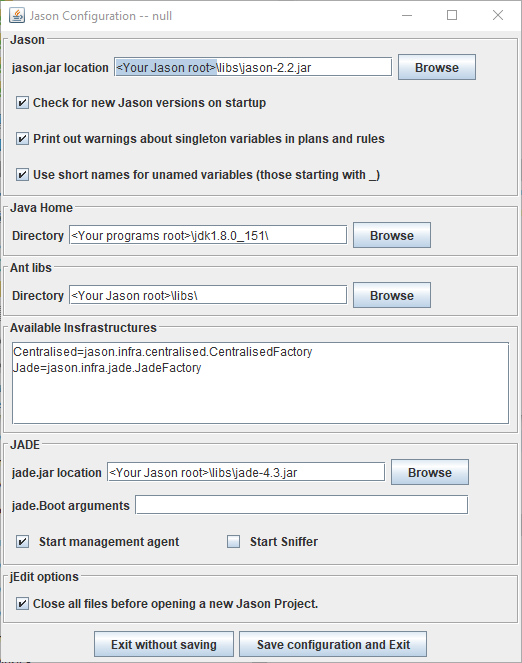
\includegraphics[width=.45\linewidth]{./figures/jason_config.png}
        \end{center}
        
\end{frame}
%/////////

%/////////
\begin{frame}[c]{[Legacy] Install \jason{} III}
        %
    \begin{enumerate}\setcounter{enumi}{4}
        
        \item now open Eclipse and click \alert{``Help $>$ Install New Software\ldots' $>$ Add..''}, then type in the ``Location'' field 
        \begin{center}
            \alert{\texttt{http://jason.sourceforge.net/eclipseplugin/juno/}}
        \end{center}
        %
        for Juno or newer \footnote{beware: this version of the plugin only works with Eclipse for Java EE, because reasons (only known to \jason{} dev team :D)}
        \begin{center}
            \alert{\texttt{http://jason.sourceforge.net/eclipseplugin/}}
        \end{center}
        for Indigo
        
        \vfill
    
        \item click ``Ok'' and wait for the ``\texttt{jasonide}'' feature to appear, then tick the checkbox and step through the installation process (Eclipse restart included)
        %
    \end{enumerate}

    \vfill
    %
\end{frame}
%/////////

\subsection{Atom IDE Setup}

%/////////
\begin{frame}[c]{Install and Configure the Atom IDE}
    
    If you care about syntax colouring in \jason{} scripts, you can rely on the Atom IDE
    %
    \vfill
    %
    \begin{itemize}
        \item download \& install Atom if not already installed
        %
        \begin{center}
            \uurl{https://atom.io}
        \end{center}
        
        \vfill
        
        \item click on \alert{``File'' menu $>$ ``Settings'' option $>$ ``Install'' section }
        
        \vfill
        
        \item then search and install the following plugins
        %
        \begin{itemize}
            \item \alert{\texttt{language-agentspeak}} to enable \jason{} syntax colouring
            \item \alert{\texttt{language-kotlin}} to enable Kotlin syntax colouring (useful for Gradle)
            \item \alert{\texttt{terminal-tab}} to enable in-IDE consoles (useful for launching Gradle tasks)
        \end{itemize}
    \end{itemize}
    
\end{frame}
%/////////

\subsection{\jason{} Exercises}

%/////////
\begin{frame}[c]{Clone/Download the Exercises}
    \begin{enumerate}	
        %
        \item clone the following repository into some directory of choice
        \begin{center}
            \uurl{https://gitlab.com/pika-lab/courses/as/ay1920/jason-agents}
        \end{center}
    
        \vfill
    
        \item open the directory of choice through your favourite IDE
        %
        \begin{itemize}
            \item import as a Gradle project, if possible (e.g. in IntelliJ or Eclipse)
        \end{itemize}
        
        \vfill
        
        \item inspect the project structure and the available Gradle tasks
    \end{enumerate}
\end{frame}
%/////////

%/////////
\begin{frame}[c]{Project Structure}

\centering
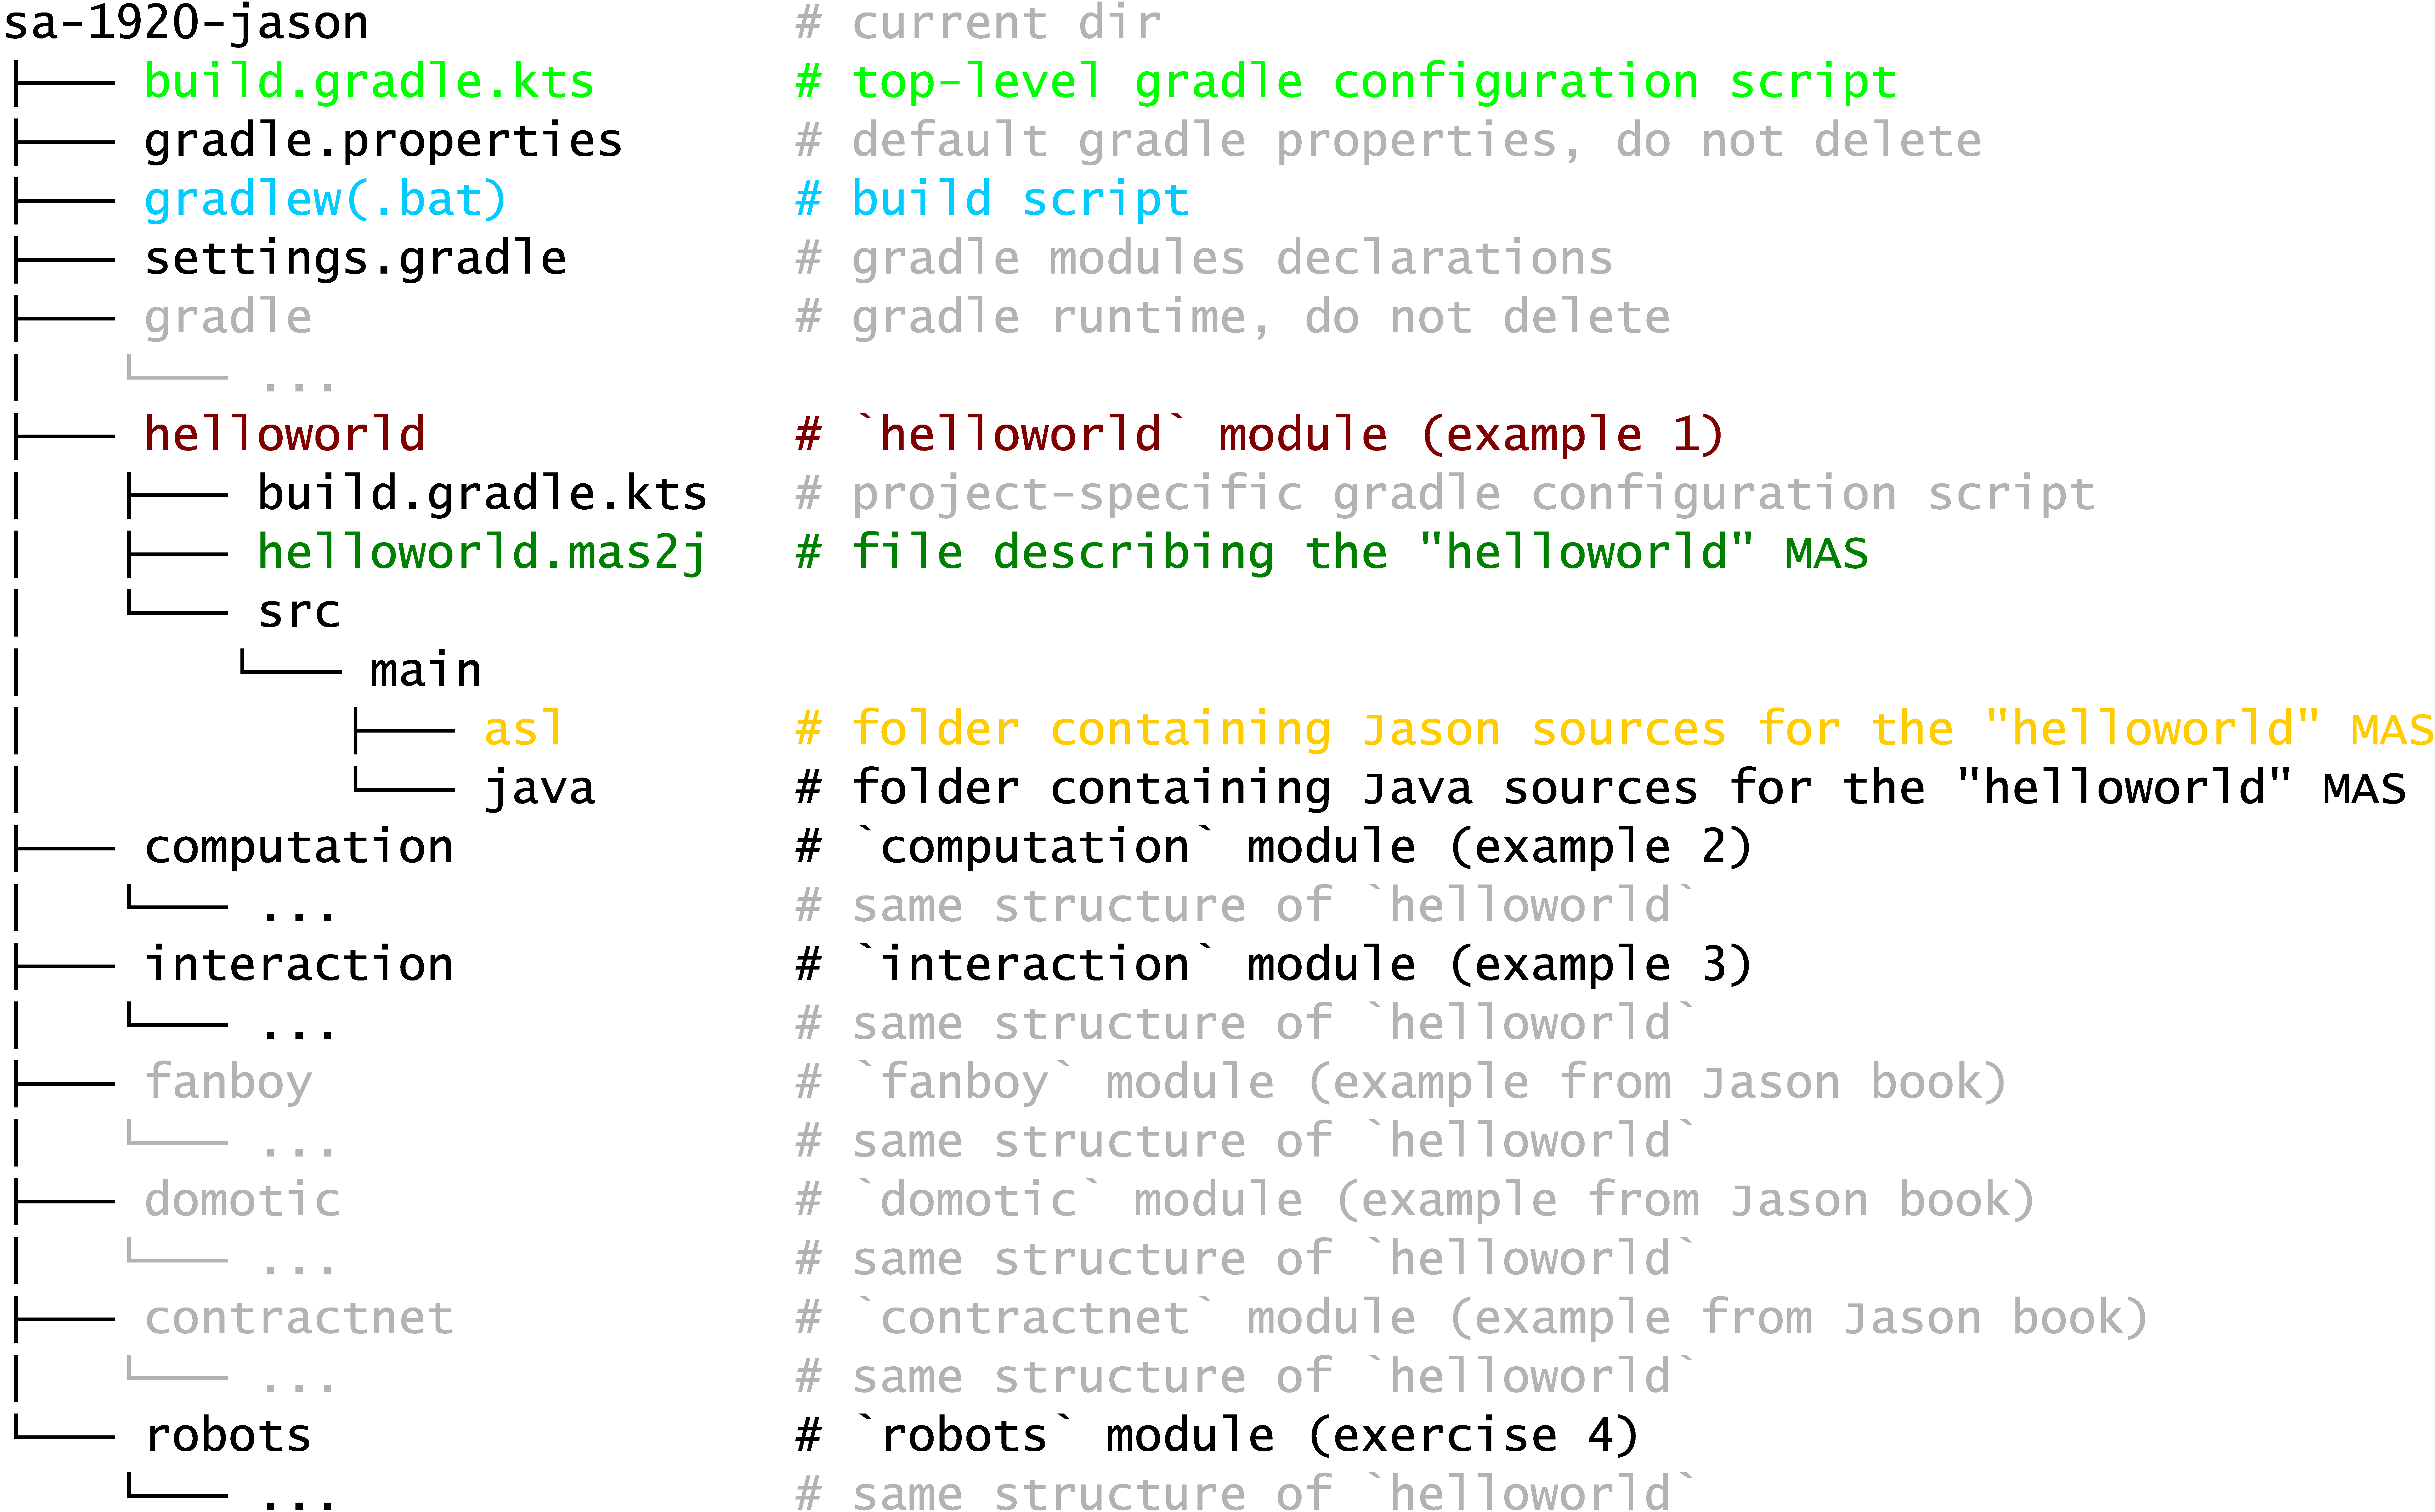
\includegraphics[width=.7\linewidth]{figures/project-structure.pdf}

\begin{block}{About Gradle tasks}
    For each file \texttt{\textit{X}.mas2j} Gradle defines a task named \alert{\texttt{run\textit{X}Mas}} which launches the corresponding \jason{} MAS
\end{block}

\end{frame}
%/////////

%===============================================================================
\section{\jason{} Basics}
%===============================================================================

\newcounter{JasonExample}
\setcounter{JasonExample}{1}

\subsection{Hello World}

%/////////
\begin{frame}[c]{Example \theJasonExample{} -- Hello World}
    
    
    \begin{itemize}
        \item consider project \texttt{:helloworld}
        
        \vfill
        
        \item have a look to \texttt{helloworld/src/main/asl/\alert{hello\_agent.asl}}
        %
        \lstinputlisting[language=Jason]{listings/hello_agent.asl}
        
        \vfill
        
        \item you can launch this example by running
        %
        \begin{itemize}
            \item[\$] \texttt{./gradlew runHelloworldMas}
        \end{itemize}
    \end{itemize}
\end{frame} 
%/////////

%/////////
\begin{frame}[c]{Example \theJasonExample{} -- Hello World \textit{(Behind the Scenes)}}
    
    
    \begin{itemize}
        \item what does the \texttt{runHelloworldMas} do?
        
        \vfill
        
        \item it launches the MAS described by \texttt{helloworld/\alert{helloworld.mas2j}}
        %
        \lstinputlisting[language=Mas2J]{listings/helloworld.mas2j}
        
        \vfill
        
        \item the \texttt{helloworld.mas2j} states a new MAS should be instantiated 
        %
        \begin{itemize}
            \item leveraging on a \emph{centralised} infrastructure%
            \footnote{distributed infrastructures are available as well, through Jade}
            
            \item containing a single agent, named \alert{\texttt{agent1}} \ldots{}
            
            \item \ldots{} whose code is the \texttt{\alert{hello\_agent}.asl} file \ldots{}
            
            \item \ldots{} which can be found within the \texttt{src/main/asl} directory
        \end{itemize}
    \end{itemize}
\end{frame} 
%/////////

%/////////
\begin{frame}[c]{The MAS Console}

    \begin{itemize}
        \item a new \alert{MAS Console} should appear, showing \texttt{agent1}'s message
        %
        \begin{center}
            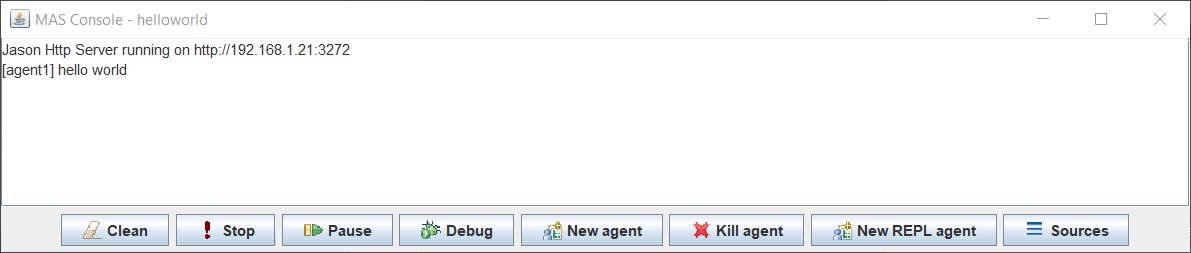
\includegraphics[width=\linewidth]{figures/mas-console.png}
        \end{center}
        
        \vfill
        
        \item notice that the console does \emph{not} disappear after \texttt{agent1} is over 
        
        \vfill
        
        \item[!] this is because \texttt{agent1} is \emph{not} over
    
        \vfill
        
        \item novel events may occur in principle, triggering some plan on \texttt{agent1}
        %
        \begin{itemize}
             \item[eg] another agent sending some message to it
             \item[eg] \ldots{} such as the user, leveraing on a REPL agent
        \end{itemize}
        
        \vfill
        
        \item[$\rightarrow$] The MAS should be explicitly closed, through the \alert{Stop} button
    \end{itemize}
\end{frame} 
%/////////

\subsection{Computation}

%/////////
\begin{frame}[c]{Computational Aspects of \jason{}}

A series of examples will follow showing how a number of computational aspects are tackled by \jason{}
%
\begin{enumerate}
    \item recursion
    \item loops
    \item conditions / guards / branches
    \item concurrency
    \item storage
\end{enumerate}

\vfill

All the examples above are provided as part of the \texttt{:computation} sub-project

\end{frame} 
%/////////

\subsubsection{Recursion}

%/////////
\stepcounter{JasonExample}
\begin{frame}[c, allowframebreaks]{Example \theJasonExample{} -- Recursion}
    \begin{itemize}
        \item recursion is the basic brick of long lasting behaviours in \jason{}
        
        \vspace{.3cm}
        
        \item consider for instance the \texttt{recursive\_agent.asl} agent
        %
        \lstinputlisting[language=Jason]{listings/recursive_agent.asl}
        
        \vspace{.3cm}
        
        \item[!] despite the syntax, those are \emph{not} method call
        %
        \begin{itemize}
            \item[$\rightarrow$] a plan for a given goal $G$ may contain $G$ in its body
        \end{itemize}
        
        \vspace{.3cm}
        
        \item other things one may note
        %
        \begin{itemize}
            \item goals may be \alert{structured} logic terms (carrying arguments)
            \item plans triggering events (i.e. heads) may contain \alert{logic variables}
            \item plan selection is performed through \alert{logical unification}
            \item \alert{eager evaluation} of sub-goals arguments ($\neq$ Prolog)
        \end{itemize}
        
        \vspace{.3cm}
        
        \item how to run this example
        %
        \begin{itemize}
            \item[\$] \texttt{./gradlew run\alert{Recursion}Mas}
        \end{itemize}
        
    \end{itemize}
\end{frame}
%/////////

\subsubsection{Loops}

%/////////
\stepcounter{JasonExample}
\begin{frame}[c, allowframebreaks]{Example \theJasonExample{} -- While Loops}
    \begin{itemize}
        \item \jason{} extends AgentSpeak(L) through imperative constructs such as \alert{while} loops, having the syntax
        %
        \begin{center}
            \texttt{while(\textit{Condition}) \{ \textit{Subgoals} \} }
        \end{center}
        
        \vspace{.3cm}
        
        \item \texttt{\textit{Subgoals}} are re-achieved as long as \texttt{\textit{Condition}} can be proved true against the belief base
        %
        \begin{itemize}
            \item through a Prolog-like resolution mechanism
        \end{itemize}
        
        \framebreak
        
        \item consider for instance the \texttt{while\_iterative\_agent.asl} agent
        %
        \lstinputlisting[language=Jason]{listings/while_iterative_agent.asl}
        
        \vspace{.3cm}
        
        \item some subgoal in \texttt{\textit{Subgoals}} may be used to alter the belief base
        %
        \begin{itemize}
            \item this is how one can break the loop
        \end{itemize}
        
        \framebreak
        
        \item other things one may note
        %
        \begin{itemize}
            \item semicolons separate subgoals, they are not simply put at the end of a subgoal
            \item dots always terminate plans
        \end{itemize}
        
        \vspace{.3cm}
        
        \item how to run this example
        %
        \begin{itemize}
            \item[\$] \texttt{./gradlew run\alert{WhileIteration}Mas}
        \end{itemize}
        
    \end{itemize}
\end{frame}
%/////////

%/////////
\stepcounter{JasonExample}
\begin{frame}[c, allowframebreaks]{Example \theJasonExample{} -- For-Each Loops}
    \begin{itemize}
        \item \jason{} extends AgentSpeak(L) through imperative constructs such as \alert{for-each} loops as well, having the syntax
        %
        \begin{center}
            \texttt{for(\textit{Query}) \{ \textit{Subgoals} \} }
        \end{center}
        
        \vspace{.3cm}
        
        \item \texttt{\textit{Subgoals}} are repeated once for each possible of way of solving \texttt{\textit{Query}} against the agent's belief base
        %
        \begin{itemize}
            \item in a lazy way (starting from \jason{} 2.5\footnote{\url{https://github.com/jason-lang/jason/issues/39}})
        \end{itemize}
        
        \vspace{.3cm} 
        
        \item consider for instance the \texttt{foreach\_iterative\_agent.asl} agent
        %
        \lstinputlisting[language=Jason]{listings/foreach_iterative_agent.asl}
        
        \vspace{.3cm}
        
        \item other things one may note
        %
        \begin{itemize}
            \item an agent's belief base can contain Prolog-like \alert{rules}
            \item testing a query against the belief base may involve \alert{backtracking} 
            \item the exemplified agent essentially attempts to print all \alert{Peano numbers}
        \end{itemize}
        
        \vspace{.3cm}
        
        \item how to run this example
        %
        \begin{itemize}
            \item[\$] \texttt{./gradlew run\alert{ForEachIteration}Mas}
        \end{itemize}
        
    \end{itemize}
\end{frame}
%/////////

\subsubsection{Guards, Conditions, and Branches}

%/////////
\stepcounter{JasonExample}
\begin{frame}[c, allowframebreaks]{Example \theJasonExample{} -- Plans Guards}
    \begin{itemize}
        \item plans in AgentSpeak(L) may optionally expose \alert{guards}
        %
        \begin{itemize}
            \item a missing guard defaults to \texttt{true}
        \end{itemize}
        
        \vspace{.3cm}
        
        \item guards are used to \alert{select} which variants of a plan the deliberation process may select 
        
        \vspace{.3cm} 
        
        \item consider for instance the \texttt{finitely\_recursive\_agent.asl} agent
        %
        \lstinputlisting[language=Jason]{listings/finitely_recursive_agent.asl}
        
        \vspace{.3cm}
        
        \item other things one may note
        %
        \begin{itemize}
            \item trivial conditions may be denoted through logic variables alone (e.g. \texttt{start(N, N)})
        \end{itemize}
        
        \vspace{.3cm}
        
        \item how to run this example
        %
        \begin{itemize}
            \item[\$] \texttt{./gradlew run\alert{FiniteRecursion}Mas}
        \end{itemize}
        
    \end{itemize}
\end{frame}
%/////////


%/////////
\stepcounter{JasonExample}
\begin{frame}[c, allowframebreaks]{Example \theJasonExample{} -- If-Then-Else Statements}
    \begin{itemize}
        \item \jason{} extends AgentSpeak(L) through imperative constructs such as \alert{if-then} or  \alert{if-then-else} statements, having the syntax
        %
        \begin{center}
            \texttt{if(\textit{Condition}) \{ \textit{ThenGoals} \} \alert{[} else \{ ElseGoals \}  \alert{]}}
        \end{center}
        %
        (where square brackets denote optionality)
        
        \vspace{.3cm}
        
        \item the behaviour of such statements is similar to how if-then(-else) constructs work in imperative languages such as Java
        
        \framebreak
        
        \item consider for instance the \texttt{conditional\_agent.asl} agent
        %
        \lstinputlisting[language=Jason]{listings/conditional_agent.asl}
        
        \framebreak
        
        \item other things one may note
        %
        \begin{itemize}
            \item trivial conditions may be denoted through logic variables alone (e.g. \texttt{start(N, N)})
        \end{itemize}
        
        \vspace{.3cm}
        
        \item how to run this example
        %
        \begin{itemize}
            \item[\$] \texttt{./gradlew run\alert{Conditions}Mas}
        \end{itemize}
        
    \end{itemize}
\end{frame}
%/////////

%/////////
\stepcounter{JasonExample}
\begin{frame}[c, allowframebreaks]{Exercise \theJasonExample{} -- Pure AgentSpeak(L) Plans}
    \begin{itemize}
        \item let's practice with pure AgentSpeak(L) Plans
        
        \vspace{.3cm}
        
        
        \item consider the (empty) file \texttt{guarded\_agent.asl}
        
        \vspace{.3cm}
        
        \item fill it with some \alert{pure} AgentSpeak(L) code, making the agent behave \emph{exactly} as the aforementioned \texttt{conditional\_agent.asl} agents (in terms of printed lines)
        
        \vspace{.3cm}
        
        \item notice that pure AgentSpeak(L) Plans cannot rely on if-then(-else) statements, nor loops
        %
        \begin{itemize}
            \item only recursion and guards are allowed
        \end{itemize}
        
        \vspace{.3cm}
        
        \item how to run this exercise
        %
        \begin{itemize}
            \item[\$] \texttt{./gradlew run\alert{Guards}Mas}
        \end{itemize}
        
    \end{itemize}
\end{frame}
%/////////

\subsubsection{Plan Failures}

%/////////
\stepcounter{JasonExample}
\begin{frame}[c, allowframebreaks]{Example \theJasonExample{} -- Failures}
    \begin{itemize}
        \item \jason{} extends AgentSpeak(L) with a particular notation aimed at dealing with failed plans, having the syntax 
        %
        \begin{center}
            \texttt{\alert{-}\textit{Event} \alert{[} : \textit{Guard} \alert{]} <- \textit{Body} .}
        \end{center}
        %
        (where square brackets denote optionality)
        
        \vspace{.3cm}
        
        \item in essence, \jason{} allows for failure plans, i.e., plans aimed at intercepting the failure of other plans
        
        \vspace{.3cm}
        
        \item whenever a \jason{} agents fails in achieving some \texttt{\textit{Goal}}, a failure event \texttt{\alert{-}\textit{Goal}} is generated, and an attempt is made to select a plan for it
        %
        \begin{itemize}
            \item plan selection in this case works as usual, by looking for a plan whose head matches \texttt{\alert{-}\textit{Goal}}, and whose guard is true
            \item is no such a plan if found the whole intention is interrupted and an error message is logged on the console
        \end{itemize}
        
        \vspace{.3cm}
        
        \item keep in mind the following conceptual equations
        %
        \[
            \begin{array}{rcccccl}
                \text{exception} & : & \text{thread} & \approx & \text{failure event} & : & \text{intention} 
                \\
                \text{exception} & : & \text{try-catch} & \approx & \text{failure event} & : & \text{minus-headed plan}
            \end{array}
        \]
        
        \vspace{.3cm}
        
        \item[!] technically, intentions are \alert{not} threads in the current \jason{} implementation
        
        \framebreak
        
        \item consider for instance the \texttt{failing\_agent.asl} agent
        %
        \lstinputlisting[language=Jason]{listings/failing_agent.asl}
        
        \vspace{.3cm}
        
        \item the agent is a gambler, it keeps throwing a fair coin until it fails
        %
        \begin{itemize}
            \item it fails if it gets cross 
            \item when this happens, an error message is logged by the interpreter
        \end{itemize}
        
        \vspace{.3cm}
        
        \item failure handling plans can be used to avoid error messages
        %
        \lstinputlisting[language=Jason]{listings/failing_agent.delta.asl}
        
        \vspace{.3cm}
        
        \item the gambler agent can now retry up to a given amount of times
        %
        \begin{itemize}
            \item after that, it terminates the gambling activity \alert{gracefully}
        \end{itemize}
        
        \framebreak
        
        \item other things one may note
        %
        \begin{itemize}
            \item in failure handling plans, retrials must be spiecified \alert{explicitly}
            \item the \alert{\texttt{.random}/1} internal action, extracting random real numbers in $\left[0,1\right[$
            \item the \alert{\texttt{.fail}/0}, making the current plan fail
        \end{itemize}
        
        \vspace{.3cm}
        
        \item how to run this example
        %
        \begin{itemize}
            \item[\$] \texttt{./gradlew run\alert{Failure}Mas}
        \end{itemize}
        
    \end{itemize}
\end{frame}
%/////////

\subsubsection{Intentions}

%/////////
\stepcounter{JasonExample}
\begin{frame}[c, allowframebreaks]{Example \theJasonExample{} -- Multiple Initial Goals}
    \begin{itemize}
        \item AgentSpeak(L) agents can have multiple \alert{intentions} at a time
        
        \vspace{.3cm}
        
        \item intentions are executed concurrently thanks to the agent's internal scheduling
        %
        \begin{itemize}
            \item which, by default, works in a cooperative, Round-Robin-like fashion
            \item notice that, behind the scenes, intention $\neq$ thread
        \end{itemize}
        
        \vspace{.3cm}
        
        \item in the general case, intentions are \alert{interleaved} at the sub-goal level
        %
        \begin{itemize}
            \item actions and internal actions execution is \alert{atomic}
            \item plan selection is atomic
            %
            \begin{itemize}
                \item thus, guards evaluation is atomic as well
            \end{itemize}
            \item belief insertion, access, or removal is atomic
            \item intention-related operations (e.g. adding/removing a sub-goal) are atomic
            \item anything else is not atomic
        \end{itemize}
        
        \vspace{.3cm}
        
        \item an easy way to create a multi-intention agent is by endowing it with multiple \alert{initial goals}
        
        \vspace{.3cm}
        
        \item consider for instance the \texttt{multi\_goals\_agent.asl} agent
        %
        \lstinputlisting[language=Jason]{listings/multi_goals_agent.asl}
        
        \vspace{.3cm}
        
        \item the agent is \alert{simultanously} counting from 0 up to 10 and from 100 down to 90
        %
        \begin{itemize}
            \item as you can see, printed lines are interleaved
        \end{itemize}
        
        \vspace{.3cm}
        
        \item how to run this example
        %
        \begin{itemize}
            \item[\$] \texttt{./gradlew run\alert{MultiGoals}Mas}
        \end{itemize}
        
    \end{itemize}
\end{frame}
%/////////

%/////////
\stepcounter{JasonExample}
\begin{frame}[c, allowframebreaks]{Example \theJasonExample{} -- Spawning New Intentions}
    \begin{itemize}
        \item \jason{} agents can spawn new intentions while executing a plan.
        %
        This can be done through the following syntax
        %
        \begin{center}
            \texttt{\alert{!!}\textit{SubGaol}}
        \end{center}
        %
        which generates an event \texttt{+!SubGoal} to be ``served'' by a newly created intentions.
        
        \vspace{.3cm}
        
        \item remember that intentions are essentially lightweight threads which are internal w.r.t. an agent
        
        \vspace{.3cm}
        
        \item new new intention is then executed concurrently w.r.t. all the pre-existing intentions
        
        \framebreak
        
        \item consider for instance the \texttt{multi\_intentions\_agent.asl} agent
        %
        \lstinputlisting[language=Jason]{listings/multi_intentions_agent.asl}
        
        \framebreak
        
        \item the agent starts by counting from 1 up to 10
        %
        \begin{itemize}
            \item as soon as it reaches 7, it starts another counting from 1 up to 10
            %
            \begin{itemize}
                \item as soon as it reaches 7, it starts another counting from 1 up to 10
                \\
                \hspace{.5cm} \ldots{}
            \end{itemize}
        \end{itemize}
        %
        \begin{center}
            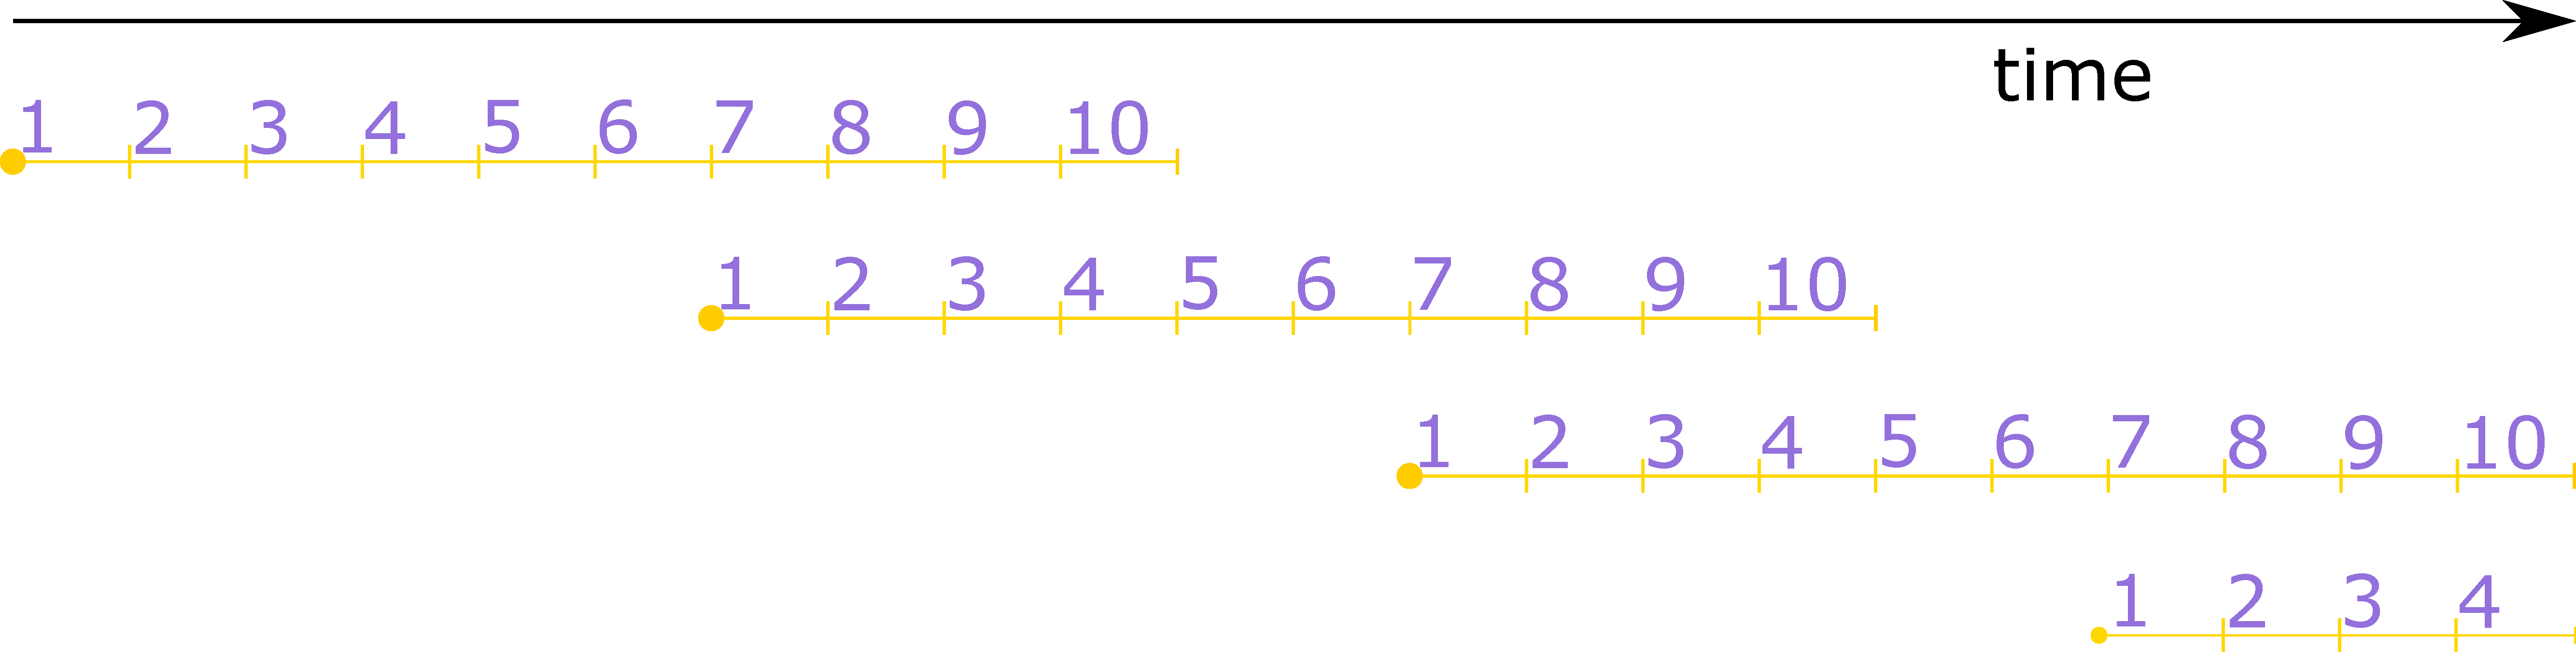
\includegraphics[width=\linewidth]{figures/multi-intentions.pdf}
        \end{center}
        
        \framebreak
        
        \item in this way, the agent can create an \alert{infinite} computation, by only leveraging on small, \alert{finite} rounds, executed on different intentions
        %
        \begin{itemize}
            \item[!] this is the preferred way to implement long-lasting \& recursive computations while keeping the intention \alert{stack size} small 
        \end{itemize}
        
        \vspace{.3cm}
        
        \item how to run this example
        %
        \begin{itemize}
            \item[\$] \texttt{./gradlew run\alert{MultiIntentions}Mas}
        \end{itemize}
        
    \end{itemize}
\end{frame}
%/////////

\subsubsection{Internal Actions}

%/////////
\begin{frame}[c, allowframebreaks]{\jason{} Internal Actions}
    \begin{itemize}
        \item \jason{} extends AgentSpeak(L) with a particular syntax for \alert{internal actions}, that is
        %
        \begin{center}
            \texttt{\alert{.}\textit{internal\_action\_name}\alert{[}(Arg$_1$, Arg$_2$, \ldots)\alert{]}}
        \end{center}
        %
        where square brackets denote optionality
        
        \vspace{.3cm}
        
        \item you have already been using some of them, such as
        %
        \begin{itemize}
            \item \texttt{\alert{.print}/*} | aimed at outputting strings on the console
            \item \texttt{\alert{.wait}/1} | aimed at waiting a given amount of time (in milleseconds)
            \item \texttt{\alert{.fail}/0} | provoking the current plan failure
            \item \texttt{\alert{.random}/1} | retrieving a random number in $\left[ 0, 1 \right[$
        \end{itemize}
        
        \vspace{.3cm}
        
        \item there exist many other internal actions in \jason{} Standard Library, and there exists other use cases for the ones you already know.
        %
        These are described at
        %
        \begin{center}
            \uurl{http://jason.sourceforge.net/api/jason/stdlib/package-summary.html}
        \end{center}
    
        \vspace{.3cm}
        
        \item however, developers may write their own internal actions, in Java, by extending the \href{http://jason.sourceforge.net/api/jason/asSemantics/DefaultInternalAction.html}{\texttt{ason.asSemantics.\alert{DefaultInternalAction}}} class
        %
        \begin{itemize}
            \item which is part of \jason{} runtime
        \end{itemize}
    
        \vspace{.3cm}
        
        \item custom internal actions can be referenced in \texttt{.asl} files through the following extended syntax
        %
        \begin{center}
            \texttt{\alert{package.of.}\textit{internal\_action\_class\_name}\alert{[}(Arg$_1$, Arg$_2$, \ldots)\alert{]}}
        \end{center}
    
        \vspace{.3cm}
        
        \item consider for instance the \texttt{utils.rand\_int} Java class
        %
        \lstinputlisting[language=Java]{listings/rand_int.java}
        
        \vspace{.3cm}
        
        \item it implements the \texttt{utils.rand\_int(-Value, +Min, +Max)} internal action, drawing a random integer value from the $\left[\mathtt{Min}, \mathtt{Max}\right[$, and binding it to the first argument	
        
    \end{itemize}
\end{frame}
%/////////

\subsubsection{Test Goals}

%/////////
\stepcounter{JasonExample}
\begin{frame}[c, allowframebreaks]{Example \theJasonExample{} -- Test Goals}
    \begin{itemize}
        \item so far, we only used \alert{achievement} goals, which are aimed at supporting agents' pragmatic actions
        
        \vspace{.3cm}
        
        \item however, AgentSpeak(L) agents can also pursue \alert{test} goals, which are aimed at supporting agents' epistemic actions
        
        \vspace{.3cm}
        
        \item while achievement goals are \texttt{!}-prefixed, test goals are \texttt{?}-prefixed
        
        \vspace{.3cm}
        
        \item test goal essentially work similarly to achievement goals, except that
        %
        \begin{itemize}
            \item when a plan for a given test goal \texttt{?Goal} is missing\ldots{}
            \item \ldots{} then \texttt{Goal} is tested against the belief-base\ldots{}
            \item \ldots{} and only if the latter operation fails, a failure event \texttt{-?Goal} is raised
        \end{itemize}
        
        \framebreak
        
        \item consider for instance the \texttt{bingo\_agent.asl} agent
        %
        \lstinputlisting[language=Jason]{listings/bingo_agent.asl}
        
        \vspace{.3cm}
        
        \item the agent keeps drawing random numbers from the $\{1, \ldots, 90 \}$ set, retrying if a number has been already extracted
        %
        \begin{itemize}
            \item notice that while there exist an explicit plan for the \texttt{?extract\_new(X)} test goal,
            \item there is no plan for \texttt{?not(extracted(X))}, yet it works
        \end{itemize}
    
        \vspace{.3cm}
    
        \item other things one may note
        %
        \begin{itemize}
            \item rules in \jason{} belief-bases support negation as failure\footnote{\url{https://en.wikipedia.org/wiki/Negation_as_failure}} through \texttt{not/1}
            \item the number extraction algorithm requires more and more time: its strategy is inadequate for Bingo
        \end{itemize}
        
        \vspace{.3cm}
        
        \item how to run this example
        %
        \begin{itemize}
            \item[\$] \texttt{./gradlew run\alert{Bingo}Mas}
        \end{itemize}
        
    \end{itemize}
\end{frame}
%/////////

\subsubsection{A Complete Example: Fibonacci sSequence}

%/////////
\stepcounter{JasonExample}
\begin{frame}[c, allowframebreaks]{Example \theJasonExample{} -- Fibonacci Sequence \textit{(dummy impl.})}
    \begin{itemize}
        \item let's provide a full-fledged computational example: an agent computing the Fibonacci sequence
        
        \vspace{.3cm}
        
        \item consider for instance the \texttt{dummy\_fibonacci\_agent.asl} agent
        %
        \lstinputlisting[language=Jason]{listings/dummy_fibonacci_agent.asl}
        
        \vspace{.3cm}
        
        \item notice that the computation of \texttt{fib(N, F)} progressively slows down as \texttt{N} increases
         %
         \begin{itemize}
             \item the current implementation is indeed quite dummy: no previously computed valued is re-used
         \end{itemize}
        
        \vspace{.3cm}
        
        \item how to run this example
        %
        \begin{itemize}
            \item[\$] \texttt{./gradlew run\alert{DummyFibonacci}Mas}
        \end{itemize}
        
    \end{itemize}
\end{frame}
%/////////

%/////////
\stepcounter{JasonExample}
\begin{frame}[c, allowframebreaks]{Exercise \theJasonExample{} -- Fibonacci Sequence}
    \begin{itemize}
        \item let's practice with pure computation in \jason{}
        
        \vspace{.3cm}
        
        \item consider the (empty) file \texttt{smart\_fibonacci\_agent.asl}
        
        \vspace{.3cm}
        
        \item fill it with some \jason{} code, making the agent behave \emph{exactly} as the aforementioned \texttt{dummy\_fibonacci\_agent.asl} agents (in terms of printed lines), while making it more efficient
        %
        \begin{itemize}
            \item try to exploit the agent belief base to cache previously computed values of the Fibonacci sequence
        \end{itemize}
        
        \vspace{.3cm}
        
        \item how to run this exercise
        %
        \begin{itemize}
            \item[\$] \texttt{./gradlew run\alert{Fibonacci}Mas}
        \end{itemize}
        
    \end{itemize}
\end{frame}
%/////////

\subsection{Interaction}

%/////////
\begin{frame}[c]{Interactive Aspects of \jason{} Agents}

A series of examples will follow showing how a number of interactive aspects are tackled by \jason{}
%
\begin{itemize}
    \item asynchronous message passing
    \item synchronous message passing
    \item broadcasting
    \item illocutionary forces of \jason{} messages
\end{itemize}

\vfill

All such examples are provided as part of the \texttt{:interaction} sub-project

\end{frame} 
%/////////

%/////////
\begin{frame}[c,allowframebreaks]{On Interaction-related Internal Actions}

Let's recall some important aspects concerning standard internal actions

\begin{itemize}
    \item the \texttt{.send/3} and \texttt{.send/5} internal actions are the basic bricks of point-to-point interactions in \jason{}
    %
    \begin{itemize}
        \item \uurl{http://jason.sourceforge.net/api/jason/stdlib/send.html}
    \end{itemize}
\end{itemize}

\begin{block}{\texttt{.send(ReceiverID, ILF, Message \textbf{[}, Answer, Timeout \textbf{]})}}
    \begin{description}
        \item[\texttt{ReceiverID}] is the name of receiver agent
        \item[\texttt{ILF}] is the illocutionary force of the message
        \item[\texttt{Message}] is the payload the message
        \item[\texttt{Answer}\footnote{\label{optArgNote}optional argument only making sense if \texttt{ILF} is \texttt{askOne}, \texttt{askAll}, or \texttt{askHow}}] the answer of an ask message, provided by the receiver
        \item[\texttt{Timeout}$^{\text{\ref{optArgNote}}}$] is the timeout (in milliseconds) when waiting for an ask answer 
    \end{description}
\end{block}

\framebreak

\begin{itemize}
    \item the \texttt{.broadcast/2} internal action is the next mechanism for interaction in \jason{}
    %
    \begin{itemize}
        \item \uurl{http://jason.sourceforge.net/api/jason/stdlib/broadcast.html}
    \end{itemize}
\end{itemize}

\begin{block}{\texttt{.broadcast(ILF, Message)}}
    \begin{description}
        \item[\texttt{ILF}] is the illocutionary force of the message
        \item[\texttt{Message}] is the payload the message
    \end{description}
\end{block}

\vspace{.6cm}

\begin{itemize}
    \item[!] the illocutionary force (ILF) dictates the semantic of the message for the receiver
    %
    \begin{itemize}
        \item and it is the same for both \texttt{.send} and \texttt{.broadcast}
    \end{itemize}
\end{itemize}

\framebreak

\begin{block}{About Illocutionary Forces (\texttt{ILF})}
    Let $S$ be the agent performing a \texttt{.send} internal action, and let $R$ be the receiver identified by \texttt{ReceiverID}, then
    %
    \begin{description}
        \item[\texttt{tell}] means $S$ intends $R$ to believe \texttt{Message} is true
        \item[\texttt{untell}] means $S$ intends $R$ to believe \texttt{Message} is not true
        \item[\texttt{achieve}] means $S$ requests $R$ to achieve \texttt{!Message}
        \item[\texttt{unachieve}] means $S$ requests $R$ to drop the goal \texttt{!Message}
        \item[\texttt{askOne}] means $S$ requests $R$ to test \texttt{?Message} once
        \item[\texttt{askAll}] means $S$ requests $R$ to test all answers for \texttt{?Message}
        \item[\texttt{tellHow}] means $S$ transfers plan $Message$ to $R$
        \item[\texttt{untellHow}] means $S$ wants $R$ to forget about the plan named \texttt{Message}
        \item[\texttt{askHow}] means $S$ requests $R$ to provide all its plans for goal \texttt{Message}
    \end{description}
\end{block}


\framebreak

\begin{itemize}
    \item the \texttt{.wait} internal action has actually several intended uses cases
    %
    \begin{itemize}
        \item \uurl{http://jason.sourceforge.net/api/jason/stdlib/wait.html}
    \end{itemize}
\end{itemize}

\begin{block}{Use cases of \texttt{.wait/1} and \texttt{.wait/2}}
    Assuming the internal action is call by intention $I$ of agent $A$
    \begin{description}
        \item[\texttt{.wait(Timeout)}\footnote{assuming \texttt{Timeout} is a number}] suspends $I$ for \texttt{Timeout} milliseconds
        \item[\texttt{.wait(\{ Event \})}\footnote{assuming \texttt{Event} is an event literal}] suspends the $I$ until \texttt{Event} occurs
        \item[\texttt{.wait(Query)}\footnote{assuming \texttt{Query} is a logic term}] suspends $I$ until \texttt{Query} can be proven against $A$'s belief base
        \item[\texttt{.wait(\{ Event \}, Timeout)}] suspends $I$ until \texttt{Event} occurs or fails if it does not within \texttt{Timeout} milliseconds
    \end{description}
\end{block}

\end{frame} 
%/////////

%/////////
\begin{frame}[c]{On Terms Annotations in \jason{}}

\begin{itemize}
    \item any logic term in \jason{} may optionally be \alert{annotated}
    %
    \begin{itemize}
        \item[i.e.] labelled with some metadata
        \item more info at \uurl{http://jason.sourceforge.net/doc/tech/annotations.html}
    \end{itemize}

    \vfill

    \item thus the general form of terms in \jason{} is
    %
    \begin{center}
        \texttt{Term\alert{[Ann$_1$, \ldots, Ann$_N$]}}
    \end{center}
    %
    \begin{itemize}
        \item where the \texttt{[Ann$_1$, \ldots, Ann$_N$]} part is a \alert{set} of annotations
        \item and each \texttt{Ann$_i$} is an un-annotated logic term
        \item if $N = 0$ (i.e. the set is empty), square brackets are omitted
    \end{itemize}

    \vfill

    \item keep in mind that \alert{annotations affect unification}
    
    \vfill
    
    \item roughly speaking, unification works as follows
    %
    \begin{center}
        \texttt{T$_1$[As$_1$] $unifies$ T$_2$[As$_2$]} $\Leftrightarrow$ $\exists \theta$ s.t. \texttt{T$_1 \theta = $T$_2 \theta\ \wedge\ $As$_1 \theta \subseteq $As$_2 \theta $}
    \end{center}
    %
    \begin{itemize}
        \item[i.e.] two terms unify if there exists a substitution $\theta$ making
        %
        \begin{enumerate}
            \item the two un-annotated terms equals, and 
            \item the leftmost term annotations a subset of the rightmost's ones
        \end{enumerate}
    \end{itemize}
\end{itemize}

\end{frame} 
%/////////

\subsubsection{Asynchronous Message Passing}

%/////////
\stepcounter{JasonExample}
\begin{frame}[c, allowframebreaks]{Example \theJasonExample{} -- Asynchronous Ping}
\begin{itemize}
    \item asynchronous message passing is the easiest interaction pattern in \jason{}
    %
    \begin{itemize}
        \item an agent $S$ sends a \alert{\texttt{tell}} \texttt{Message} to $R$
        \item this provokes a belief \texttt{Message[source($S$)]} to be added on $R$'s BB
        \item and a \texttt{+Message[source($S$)]} event to be raised for $R$
        \item possibly triggering an adequate plan of $R$, if any
        \item if $S$ expects a response, it must expose a similar plan for \texttt{+Response[source($R$)]}
    \end{itemize}
    
    \vspace{.3cm}
    
    \item consider for instance the \texttt{async\_pinger\_agent.asl} agent
    %
    \lstinputlisting[language=Jason]{listings/async_pinger_agent.asl}
    
    \vspace{.3cm}
    
    \item other things one may note
    %
    \begin{itemize}
        \item the sender must know the name of the receiver
        \item the sender activity must be split in at least 2 plans
    \end{itemize}
    
    \vspace{.3cm}
    
    \item how to run this example
    %
    \begin{itemize}
        \item[\$] \texttt{./gradlew run\alert{AsyncPingPong}Mas}
        \item[!] requires \texttt{async\_ponger\_agent.asl} (see next Exercise) 
    \end{itemize}
    
\end{itemize}
\end{frame}
%/////////

%/////////
\stepcounter{JasonExample}
\begin{frame}[c, allowframebreaks]{Exercise \theJasonExample{} -- Asynchronous Pong}
\begin{itemize}
    \item let's practice with asynchronous message passing in \jason{}
    
    \vspace{.3cm}
    
    \item consider the (empty) file \texttt{async\_ponger\_agent.asl}
    
    \vspace{.3cm}
    
    \item fill it with some \jason{} code, making the agent capable of answering back to the aforementioned \texttt{async\_pinger\_agent}
    %
    \begin{itemize}
        \item notice that the pinger is pro-active, while the ponger is deliberately reactive 
    \end{itemize}
    
    \vspace{.3cm}
    
    \item how to run this exercise
    %
    \begin{itemize}
        \item[\$] \texttt{./gradlew run\alert{AsyncPingPong}Mas}
    \end{itemize}
    
\end{itemize}
\end{frame}
%/////////

\subsubsection{Synchronous Message Passing}

%/////////
\stepcounter{JasonExample}
\begin{frame}[c, allowframebreaks]{Example \theJasonExample{} -- Synchronous Ping}
\begin{itemize}
    
    \item the problem with asynchronous message passing is that it forces agent programmers to decompose plans
    
    \vspace{.3cm}
    
    \item synchronous message passing can be easily attained in \jason{} through the \texttt{.wait} internal action
    %
    \begin{itemize}
        \item an agent $S$ sends a \alert{\texttt{tell}} \texttt{Message} to $R$
        \item then it waits for a \texttt{+Response[source($R$)]} event to be raised
        \begin{itemize}
            \item[i.e.] the \texttt{.wait} internal action suspends $S$'s intention until a response is received
        \end{itemize}
        \item the semantics of  \texttt{.send} on the receiver side is unaffected
    \end{itemize}
    
    \framebreak
    
    \item consider for instance the \texttt{sync\_pinger\_agent.asl} agent
    %
    \lstinputlisting[language=Jason]{listings/sync_pinger_agent.asl}
    
    \vspace{.3cm}
    
    \item other things one may note
    %
    \begin{itemize}
        \item the sender must still know the name of the receiver
        \item an explicit plan exists on the pinger, encoding the activity
        %
        \begin{enumerate}
            \item first send a ping
            \item then receive a pong
        \end{enumerate}
    \end{itemize}
    
    \vspace{.3cm}
    
    \item how to run this example
    %
    \begin{itemize}
        \item[\$] \texttt{./gradlew run\alert{SyncPingPong}Mas}
        \item[!] requires \texttt{sync\_ponger\_agent.asl} (see next Exercise) 
    \end{itemize}
    
\end{itemize}
\end{frame}
%/////////

%/////////
\stepcounter{JasonExample}
\begin{frame}[c, allowframebreaks]{Exercise \theJasonExample{} -- Synchronous Pong}
    \begin{itemize}
        \item let's practice with synchronous message passing in \jason{}
        
        \vspace{.3cm}
        
        \item consider the (empty) file \texttt{sync\_ponger\_agent.asl}
        
        \vspace{.3cm}
        
        \item fill it with some \jason{} code, making the agent capable of answering back to the aforementioned \texttt{sync\_pinger\_agent}
        %
        \begin{itemize}
            \item by leveraging on the \texttt{.wait} internal action
        \end{itemize}
        
        \vspace{.3cm}
        
        \item how to run this exercise
        %
        \begin{itemize}
            \item[\$] \texttt{./gradlew run\alert{SyncPingPong}Mas}
        \end{itemize}
        
    \end{itemize}
\end{frame}
%/////////

\subsubsection{Request-Response}

%/////////
\stepcounter{JasonExample}
\begin{frame}[c, allowframebreaks]{Example \theJasonExample{} -- AskOne Client-side}
\begin{itemize}
    
    \item a common situation in MAS is that of an agent $C$ asking some information to some other agent $S$ and expecting an answer
    %
    \begin{itemize}
        \item in such cases, the \texttt{\texttt{ask*}} ILFs help reducing the boilerplate
    \end{itemize}
    
    \vspace{.3cm}
    
    \item a synchronous, one-shot, request-response interaction among 2 agents can be easily attained in \jason{} through the \texttt{.send/5} internal action
    %
    \begin{enumerate}
        \item agent $C$ sends an \alert{askOne} \texttt{Message} to $S$
        \item the sending intention on $C$ is suspended 
        \item the event \texttt{+?Message[source($C$)]} event is raised on $S$
        \item a plan for \texttt{+?Message[source($C$)]} is successfully executed on $S$, through substitution $\theta$
        \item the suspended intention on $C$ is resumed and the 4$^{th}$ argument of \texttt{.send} is bound to \texttt{Message[source($C$)]$\theta$}
     \end{enumerate}
    
    \framebreak
    
    \item consider for instance the \texttt{client\_agent.asl} agent
    %
    \lstinputlisting[language=Jason]{listings/client_agent.asl}
    
    \framebreak
    
    \item other things one may note
    %
    \begin{itemize}
        \item the client must still know the name of the server
        \item it is sufficient for the server to expose test goals to be able to serve \texttt{ask*} requests
    \end{itemize}
    
    \vspace{.3cm}
    
    \item how to run this example
    %
    \begin{itemize}
        \item[\$] \texttt{./gradlew run\alert{ClientSerivce}Mas}
        \item[!] requires \texttt{server\_agent.asl} (see next Exercise) 
    \end{itemize}
    
\end{itemize}
\end{frame}
%/////////

%/////////
\stepcounter{JasonExample}
\begin{frame}[c, allowframebreaks]{Exercise \theJasonExample{} -- AskOne Server-side}
\begin{itemize}
    \item let's practice with request-response interactions in \jason{}
    
    \vspace{.3cm}
    
    \item consider the (empty) file \texttt{service\_agent.asl}
    
    \vspace{.3cm}
    
    \item fill it with some \jason{} code, making the agent capable of answering back to the aforementioned \texttt{client\_agent}
    %
    \begin{itemize}
        \item by leveraging test goals only
        \item[i.e.] without using the \texttt{.send} internal action
    \end{itemize}
    
    \vspace{.3cm}
    
    \item how to run this exercise
    %
    \begin{itemize}
        \item[\$] \texttt{./gradlew run\alert{ClientSerivce}Mas}
    \end{itemize}
    
\end{itemize}
\end{frame}
%/////////

\subsubsection{Broadcasting}

%/////////
\stepcounter{JasonExample}
\begin{frame}[c, allowframebreaks]{Example \theJasonExample{} -- Broadcaster}
\begin{itemize}
    
    \item a common situation in MAS is that of an agent $B$ needing to contact a number of agents it does not even know
    %
    \begin{itemize}
        \item in such cases, the \texttt{.broadcast} internal action can be used
    \end{itemize}
    
    \vspace{.3cm}
    
    \item the \texttt{.broadcast/2} internal action works as the \texttt{.send/3} one, except that 
    %
    \begin{itemize}
        \item it sends the message to all agents
        \item it is never suspended
        \item thus, a plan must always be defined on the broadcaster-side to handle responses
    \end{itemize}
    
    \framebreak
    
    \item consider for instance the \texttt{seeking\_agent.asl} agent
    %
    \lstinputlisting[language=Jason]{listings/seeking_agent.asl}
    
    \vspace{.3cm}
    
    \item other things one may note
    %
    \begin{itemize}
        \item the broadcaster can ignore the names of the receiver agents
        \item a \texttt{.mas2j} file can state multiple instances of an agent must be started
    \end{itemize}
    
    \vspace{.3cm}
    
    \item how to run this example
    %
    \begin{itemize}
        \item[\$] \texttt{./gradlew run\alert{HideAndSeek}Mas}
        \item[!] requires \texttt{hiding\_agent.asl} (see next Exercise) 
    \end{itemize}
    
\end{itemize}
\end{frame}
%/////////

%/////////
\stepcounter{JasonExample}
\begin{frame}[c, allowframebreaks]{Exercise \theJasonExample{} -- AskOne Server-side}
\begin{itemize}
    \item let's practice with broadcast-based interactions in \jason{}
    
    \vspace{.3cm}
    
    \item consider the (empty) file \texttt{hiding\_agent.asl}
    
    \vspace{.3cm}
    
    \item fill it with some \jason{} code, making the agent capable of answering back to the aforementioned \texttt{seeking\_agent}
    %
    \begin{itemize}
        \item leveraging test goals only should be sufficient
    \end{itemize}
    
    \vspace{.3cm}
    
    \item how to run this exercise
    %
    \begin{itemize}
        \item[\$] \texttt{./gradlew run\alert{HideAndSeek}Mas}
    \end{itemize}
    
\end{itemize}
\end{frame}
%/////////

%===============================================================================
\section{\jason{} Advanced}
%===============================================================================

\subsection{Perception \& Actuation}

%/////////
\begin{frame}[c]{Agent-specific Aspects of \jason{} Agents}
    
    A series of examples will follow describing how \alert{perception} and \alert{actuation} are handled in \jason{}.
    
    \vfill
    
    In particular, we show how in AgentSpeak(L) and \jason{}
    %
    \begin{itemize}
        \item perception is handled through \alert{automatic belief updates}
        \item actuation is handled through \alert{action expressions}
    \end{itemize}
    
    \vfill
    
    All such examples are provided as part of the \texttt{:thermostat} sub-project
    
\end{frame} 
%/////////

\subsubsection{Agents Perception}

%/////////
\begin{frame}[c]{Perception through Automatic Belief Updates}
    
    \begin{itemize}
        \item MAS are composed by (at least) two abstractions: agents and the \alert{environment}
        
        \vfill
        
        \item \jason{} reifies the environment abstraction into actual software
        
        \vfill
        
        \item one purpose of the environment in \jason{} is to endow agents with their \alert{percepts}
        
    \end{itemize}
    
    \vfill
    
    \begin{block}{Percepts as beliefs}
        Percepts in AgentSpeak(L) are ordinary beliefs (i.e. terms) in the form
        %
        \begin{center}
            \texttt{SensorData\alert{[source(\textit{percept})]}}
        \end{center}
        % 
        which are \alert{automatically} added by the environment into the perceiving agent's belief base
    \end{block}
    
\end{frame} 
%/////////

%/////////
\begin{frame}[c]{The two sides of perception}
    
    \begin{block}{Percepts from the \aalert{agent} point of view}
        \begin{itemize}
            \item each agent must simply \alert{assume} percepts in its belief base to be \alert{cosistent} with the environment
            \item each agent may intercept percepts \alert{variations} through \textit{ad-hoc} plans
            %
            \begin{itemize}
                \item[eg] \texttt{\alert{+}SensorData[source(\textit{percept})]}
                \item[eg] \texttt{\alert{-}SensorData[source(\textit{percept})]}
            \end{itemize}
        \end{itemize}
    \end{block}
    
    \vfill
    
    \begin{block}{Percepts from the \aalert{environment} point of view}
        \begin{itemize}
            \item each environment (also) has the \alert{responsibility} of tracking: 
            %
            \begin{center}\small\itshape
                \alert{all} the percepts of \alert{each} agent in \alert{any} given moment of MAS execution
            \end{center}
            
            \item thus designing the environment requires modelling \alert{which} percept each agent may perceive, and \alert{when}
        \end{itemize}
    \end{block}
    
\end{frame} 
%/////////

\subsubsection{Agents Actuation}

%/////////
\begin{frame}[c]{Perception through Automatic Belief Updates}
    
    \begin{itemize}
        \item MAS are composed by (at least) two abstractions: agents and the \alert{environment}
        
        \vfill
        
        \item \jason{} reifies the environment abstraction into actual software
        
        \vfill
        
        \item \alert{another} purpose of the environment in \jason{} is enable agents' \alert{actions}
        
    \end{itemize}
    
    \vfill
    
    \begin{block}{Actions as logic expressions}
        Syntactically, actions in AgentSpeak(L) are ordinary logic expressions which may occur in plans bodies.
        %
        They consist of terms in the form
        %
        \begin{center}
            \texttt{actionName\alert{[}(\textit{Arg}$_1$, \textit{Arg}$_2$, \ldots)\alert{]}}
        \end{center}
        % 
        (where square brackets denote optionality)
        %
        \begin{itemize}
            \item notice the lack for dot / plus / minus as prefix
        \end{itemize}
    \end{block}
    
\end{frame} 
%/////////

%/////////
\begin{frame}[c,allowframebreaks]{The Two Sides of Actuation}
    
    \begin{block}{Actions from the \aalert{agent} point of view}
        \begin{itemize}
            \item each agent simply \alert{assumes} some actions are available for it to use
            %
            \begin{itemize}
                \item action \alert{indicators} (i.e., functor + arity) should be known
            \end{itemize}
            
            \item each agent may \alert{perform} ($\approx$ call) any action in any plan
            
            \item actions may either \alert{fail or succeed}
            %
            \begin{itemize}
                \item failing actions provoke \alert{plans failures}
                \item succeeding actions (may) provoke \alert{side effects} on the environment
                %
                \begin{itemize}
                    \item to be eventually perceived and handled by the agent
                \end{itemize}
            \end{itemize}
            
            \item performing a ``missing'' action always provokes a failure
        \end{itemize}
    \end{block}
    
    \framebreak
    
    \begin{block}{Percepts from the \textbf{environment} point of view}
        \begin{itemize}
            \item each environment (also) has the \alert{responsibility} of exposing 
            %
            \begin{center}\small\itshape
                \alert{all} the actions of \alert{each} agent may perform in \alert{any} given moment of MAS execution
            \end{center}
            
            \item thus designing the environment also requires modelling \alert{which} actions each agent may perform, and what its \alert{effect} is
            
            \item technically, the environment is where actions are implemented
        \end{itemize}
    \end{block}
    
\end{frame} 
%/////////

\subsection{Custom Environments}

%/////////
\begin{frame}[c,allowframebreaks]{Designing \& Implementing Custom Environment}
    
    \begin{itemize}
        \item custom environments are implemented in Java by extending the class
        %
        \begin{center}
            \uurl{http://jason.sourceforge.net/api/jason/environment/Environment.html}
        \end{center}
    
        \vspace{.3cm}
    
        \item the \texttt{jason.environment.\alert{Environment}} class comes with some utility methods for agents' life cycle and belief base management, plus 3 main \alert{callbacks} to be overridden by developers
        %
        \begin{itemize}
            \item \lstinline[language=Java]{void init(String[] args)} | which is invoked once, upon MAS initialization
            \item \lstinline[language=Java]{boolean executeAction(String agentName, Structure actionTerm)} | which is invoked whenever the agent named \texttt{agentName} performs the action represented by \texttt{actionTerm}
            \item \lstinline[language=Java]{Collection<Literal> getPercepts(String agentName)} | which is invoked whenever the agent named \texttt{agentName} observes the environment
        \end{itemize}
    
        \framebreak
        
        \item the particular subclass of \texttt{Environment} to be used for a MAS must be indicated into the \texttt{.mas2j} file
        %
        \lstinputlisting[language=Mas2J]{listings/myMas.mas2j}
        %
        \begin{itemize}
            \item notice that the \texttt{arg1}, $\ldots$, \texttt{argN} arguments provided by developers to the environment in the \texttt{.mas2j} file are passed \alert{as strings} to the \texttt{init} method of the environment instance, upon start-up
        \end{itemize}
        
    \end{itemize}
    
\end{frame} 
%/////////

\subsubsection{The Thermostat Example}

%/////////
\stepcounter{JasonExample}
\begin{frame}[c, allowframebreaks]{Example \theJasonExample{} -- The Thermostat Example}
\begin{itemize}
    
    \item we present a classical example of a MAS composed by just 1 thermostat agent willing to keep the temperature of its environment close to 20 degrees
    
    \vspace{.3cm}
    
    \item we model its environment as characterised by a single observable property: \alert{temperature}
    
    \vspace{.3cm}
    
    \item we endow the thermostat agent with a \alert{temperature sensor} outputting percepts in the form \alert{\texttt{temperature(T)}}
    
    \vspace{.3cm}
    
    \item we also endow it with an \alert{actuator} for \alert{spraying} cold/hot air, in order to affect the environment temperature.
    %
    Thus, the thermostat agent can perform 2 sorts of actions
    %
    \begin{itemize}
        \item \lstinline[language=Jason]{spray_air(hot)} | which increases the temperature
        \item \lstinline[language=Jason]{spray_air(cold)} | which decreases the temperature
    \end{itemize}
    
    \vspace{.3cm}
    
    \item both actions may fail, with a given probability (20\%)
    
    \framebreak
    
    \item such design choices are reified by the following class
    %
    \lstinputlisting[language=Java]{listings/TemperatureEnvironment.java}
    
    \framebreak
    
    \item the thermostat agent is then as simple as
    %
    \lstinputlisting[language=Jason]{listings/thermostat_agent.asl}
    
    \framebreak
    
    \item other things one may note
    %
    \begin{itemize}
        \item no loop or recursion is present in the agent code
        \item the failure of action must always be taken into account
    \end{itemize}
    
    \vspace{.3cm}
    
    \item how to run this example
    %
    \begin{itemize}
        \item[\$] \texttt{./gradlew run\alert{Thermostat}Mas}
    \end{itemize}
    
\end{itemize}
\end{frame}
%/////////

\subsubsection{Visualisation of Spatial Environments}

%/////////
\begin{frame}[c]{Environment \& MVC}
    
    \begin{itemize}
        
        \item it is often the case in \jason{} that developers need a way to observe/affect a MAS through some GUI
        %
        \begin{itemize}
            \item in such cases the environment class is usually coupled with some Swing-based view
            \item which is better implemented through a separate class
        \end{itemize}
        
        \vfill
        
        \item if the environment is non-trivial, explicitly designing the \alert{model} of the environment is a best practice
        %
        \begin{itemize}
            \item in such cases the environment class is usually coupled with some model type encapsulating the state of the MAS
            \item and the admissible operations on it
            \item all such things are better reified into code through separate classes
        \end{itemize}
        
        \vfill
        
        \item technically, this resembles the Model-View-Controller (MVC)\footnote{\url{https://en.wikipedia.org/wiki/Model\%E2\%80\%93view\%E2\%80\%93controller}} pattern for GUI applications
        %
        \begin{itemize}
            \item where the environment class acts as controller
        \end{itemize}
    
        \vfill
        
        \item this is exactly how the next exercise is organised :)
        
    \end{itemize}
    
\end{frame} 
%/////////

\subsection{Rescue the Lost Robot}

%/////////
\stepcounter{JasonExample}
\begin{frame}[c, allowframebreaks]{Exercise \theJasonExample{} -- Rescue the Lost Robot}
    
    \begin{block}{Scenario}
        \begin{itemize}
            \item two robots, $R$ and $L$ are placed in a rectangular discrete environment with random poses, with no common reference frame
            
            \item robot $L$ is panicking since it has not tracked its own position
            %
            \begin{itemize}
                \item thus it feels lost and wanders randomly
            \end{itemize}
            
            \item robot $R$ is in charge of rescuing $L$
            %
            \begin{itemize}
                \item[i.e.] finding it and telling it how to go home
            \end{itemize}
            
            \item robot $R$ considers ``home'' to be its very initial position
            
        \end{itemize}
    \end{block}

    \begin{center}
        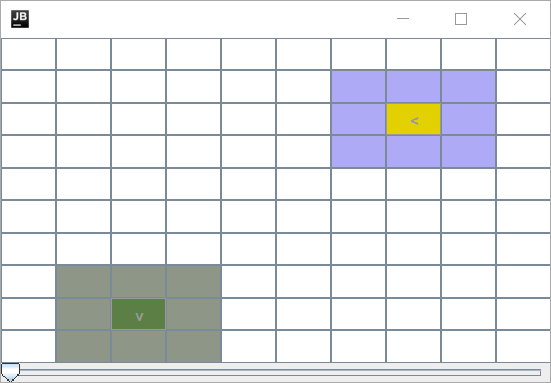
\includegraphics[width=.8\linewidth]{figures/robots.png}
    \end{center}

    \begin{exampleblock}{Constraints -- Interaction}
        \begin{itemize}
            \item robots are only allowed to send messages to each other if they are \alert{close} to each others, i.e. iff
            %
            \begin{center}
                $|x_R - x_L| \leq 1 \wedge |y_R - y_L| \leq 1$
            \end{center} 
            %
            (where $(x_R, y_R)$ and $(x_L, y_L)$ are $R$ and $L$ \alert{absolute} positions, respectively)
            
            \item broadcast is \emph{never} allowed
        \end{itemize}
    \end{exampleblock}

    \begin{exampleblock}{Constraints -- Actuation}
        \begin{itemize}
            \item robots can only \alert{move} in any of the \alert{4 relative directions} by one step at a time
            %
            \begin{itemize}
                \item[i.e.] \texttt{forward}, \texttt{backward}, \texttt{left}, and \texttt{right}
            \end{itemize}
        
            \item robots' attempts to move may fail due to a \alert{slippery floor} or an \alert{obstacle}
            %
            \begin{itemize}
                \item the \alert{sliding probability} is a parameter of the system, and it never varies during execution
                
                \item obstacles may be either the arena borders or other robots
            \end{itemize}
            
        \end{itemize}
    \end{exampleblock}

    \begin{exampleblock}{Constraints -- Perception}
        \begin{itemize}
            \item each robot $X$ can perceive the \alert{presence} of any other robot $Y$, if the two are close
            %
            \begin{itemize}
                \item in this case, a \texttt{neighbour($X$)} (resp. \texttt{neighbour($Y$)}) percept appears on $Y$'s (resp. $X$'s) belief base
            \end{itemize}
        
            \item each robot $X$ can perceive the presence/lack of \alert{obstacles} or \alert{other robots} in the 8 positions around its current one
            %
            \begin{itemize}
                \item through 8 percepts having one of the following 3 forms
                %
                \begin{center}
                    \texttt{free($Direction$)} or \texttt{obstacle($Direction$)} or \texttt{robot($Direction$)}
                \end{center}
                %
                where $Direction$ is any of \texttt{forward}, \texttt{forward\_left}, \texttt{forward\_right}, \texttt{left}, \texttt{right}, \texttt{backward}, \texttt{backward\_left}, and \texttt{backward\_right}
            \end{itemize}
        \end{itemize}
    \end{exampleblock}

    \begin{alertblock}{Requirements}
        \begin{enumerate}
            \item $L$ is keeps randomly wandering around the arena
            
            \item $R$ keeps wandering around the arena as well, looking for other agents
            %
            \begin{itemize}
                \item keeping track of its own pose through believes
            \end{itemize}
            
            \item as soon as $R$ finds $L$ \ldots
            %
            \begin{itemize}
                \item[i.e.] as soon as $R$ perceives $L$, since $R$ and $L$ are close \ldots
            \end{itemize}
        
            \item \ldots $R$ must give $L$ enough information to reach home
            
            \item the scenario is over as soon as $L$ reaches home
        \end{enumerate}
    \end{alertblock}
    
\end{frame} 
%/////////

\subsubsection{Suggestions}

%/////////
\begin{frame}[c, allowframebreaks]{Rescue the Lost Robot -- The Environment Model}
    \begin{itemize}
        \item the \texttt{\alert{Arena2DModel}} interface is aimed at keeping track \& constraining the state of the environment and the agents situated in it
        
        \vspace{.3cm}

        \item for instance, it keeps track of agents poses (absolute position + absolute orientation)
        
        \vspace{.3cm}
        
        \item furthermore, it provides facilities for 
        %
        \begin{itemize}
            \item computing agents' perceptions
            \item checking whether two agents are close to each others
        \end{itemize}
    
        \vspace{.3cm}
        
        \item its implementation is completely provided
        
        \framebreak
        
        \item an overview of its main methods is provided below:
        %
        \lstinputlisting[language=Java]{listings/Arena2DModel.java}
    
    \end{itemize}

\end{frame} 
%/////////

%/////////
\begin{frame}[c, allowframebreaks]{Rescue the Lost Robot -- The Environment}
    \begin{itemize}
        \item the \texttt{\alert{Arena2DEnvironment}} class is where agents' perception and actuation is implemented
        %
        \begin{itemize}
            \item by leveraging on some instance of \texttt{Arena2DModel}
        \end{itemize}
        
        \vspace{.3cm}
        
        \item its implementation is up to you
        
        \vspace{.3cm}
        
        \item an overview of its main structure is provided below:
        %
        \lstinputlisting[language=Java]{listings/Arena2DEnvironment.java}
        
    \end{itemize}
    
\end{frame} 
%/////////

%/////////
\begin{frame}[c]{Rescue the Lost Robot -- Internal Actions}
    \begin{itemize}
        \item the \texttt{\alert{utils}.*} package includes a number of internal actions aimed at easing agents' reasoning
        
        \vspace{.3cm}
        
        \item for instance \texttt{rand\_int(-X, +Min, +Max)} lets an agent draw random integers given a range
        
        \vspace{.3cm}
        
        \item for instance \texttt{update\_pose(+Direction)} lets an agent update its believed pose after it performed a step in a given \texttt{Direction}
        %
        \begin{itemize}
            \item notice that this internal action both reads and updates the calling agents' belief base
        \end{itemize}
        
    \end{itemize}
    
\end{frame} 
%/////////

%===============================================================================
\section{Examples from the \jason{} Book}
%===============================================================================

\subsection{Fanboy}

%/////////
%\begin{frame}[c]{Import \jason{} Project}
%	%
%	\begin{itemize}
%		%
%		\item go to 
%		\begin{center}
%			\uurl{http://apice.unibo.it/xwiki/bin/view/Courses/Sa1617Lab}
%		\end{center}
%		and download \alert{\texttt{sa1617\_agentSpeakL.zip}}
%		%
%		\item unzip it anywhere you want
%		%
%		\item in Eclipse, since the import feature of \jason{} plugin is broken\footnote{Dunno why, waiting for an answer from devs}, do the following
%			\begin{enumerate}
%				\item \emph{copy} the .mas2j file somewhere
%				\item create a new \jason{} project and name it \emph{exactly} as the project you would import
%				\item the codebase and project structure gets correctly parsed, but the .mas2j file \emph{does not}
%				\item \emph{overwrite} the new (wrong) .mas2j file with the one previously copied
%			\end{enumerate}
%		%
%	\end{itemize}
%	%
%\end{frame} 
%/////////

%/////////
\begin{frame}[c]{[Legacy] Example -- \agentspeakl{} vs.\ \jason{} I}
    %
    \begin{itemize}
        %
        \item consider now project \alert{\texttt{fanboy}}
        %
        \vfill
        %
        \item it is a very basic example of \agentspeakl{} program featuring
        %
        \begin{itemize}
            %
            \item achievement-goal addition events
            %
            \item belief addition events
            %
            \item plan contexts
            %
            \item test-goals
            %
        \end{itemize}
        %
        \vfill
        %
        \begin{block}{Can you spot what should \textbf{not} be in an \agentspeakl{} program?}
            Notice that this is a valid \jason{} program\ldots{}
        \end{block}
        %
        \vfill
        %
        \item listen to the teacher explaining the source code
        %
    \end{itemize}
\end{frame} 

%/////////
\begin{frame}[c]{[Legacy] Example -- \agentspeakl{} vs.\ \jason{} II}
    
    \begin{block}{Consider the guard of the plan for \texttt{+!book\_tickets(A,D,V)}}
        \begin{itemize}
            \item what is its meaning?
            \item change it in such a way the plan can be selected if the phone is \alert{\emph{certainly not}} busy
        \end{itemize}
    \end{block}
\end{frame} 

%/////////
\begin{frame}[c]{[Legacy] Example -- \agentspeakl{} vs.\ \jason{} III}
    \begin{block}{Edit the MAS as described below}
        \begin{itemize}
            \item the phone is shared by \alert{\texttt{fanboy}} and its \alert{\texttt{mum}}: they may compete for using the phone
            \item \texttt{mum} simply randomly tries to use the phone to call her friends \begin{itemize}
                \item when she gets the phone she keeps talking for a while
                \item \uurl{http://jason.sourceforge.net/api/jason/stdlib/random.html}
            \end{itemize}
            \item every agent getting the phone must first of all inform the other one that the phone is busy \begin{itemize}
                \item \uurl{http://jason.sourceforge.net/api/jason/stdlib/send.html}
            \end{itemize}
            \item every agent must inform the other one that the phone is not busy anymore when it ends the call
            \item every agent must wait for the phone to be free in case it is needed
            \item the phone is initially reserved by \texttt{mum}
        \end{itemize}
    \end{block}
\end{frame} 
%/////////

\subsection{Domestic Robot}

%/////////
\begin{frame}[c]{[Legacy] Example -- Domestic Robot}
    %
    \begin{enumerate}
        %
        \item consider now project \alert{\texttt{:domotic}}
        %
    
    %
%	\begin{block}{Domestic robot}
        %
        \begin{itemize}
            %
            \item a domestic robot has the goal of serving beer to its owner
            %
            \item thus, it receives beer requests from the owner, goes to the fridge, takes out a beer, brings it back to the owner
            %
            \item the robot eventually orders beer using a nearby supermarket's home delivery service
            %
            \item also, the robot obeys hard-wired rules from the Department of Health (e.g. ``do not serve more than 10 beers a day'')
            %
        \end{itemize}
    
        \vfill
        
        \item listen to the teacher explaining the source code
        %
    \end{enumerate}
    %
\end{frame} 
%/////////

%/////////
\begin{frame}[c]{Highlights}
    %
    \begin{itemize}
        %
        \item the robot should remember if beer is available irrespective of its location in the environment, because the \alert{perception} about beer stock is available \emph{only when the robot is in front of the open fridge}---as soon as it closes the fridge, the perception is gone
        
        \vfill
        
        \item how to ensure that the robot will respond \emph{only} to its owner's requests?
        
        \vfill
        
        \item what happens if we change the order of \texttt{+!at(robot, P)} plans? And if we drop the \emph{plan context} from either one? Again, what happens if we change plans order in this case?
        
        \vfill
        
        \item how to ensure each external action is available only to the right agent?
        %
    \end{itemize}
    %
\end{frame} 
%/////////

\subsection{ContractNet Protocol}

%/////////
\begin{frame}[c]{[Legacy] Example -- ContractNet Protocol}
    %
    \begin{enumerate}
        %
        \item consider now project \alert{\texttt{contractnet}}
        %
        \begin{itemize}
            %
            \item one agent, called ``initiator'', wishes to have some tasks performed, thus asks other agents, called ``participants'', to bid to perform that task
            %
            \item this asking message is called ``call for proposals'' (cfp, for short), and participants may reply by either sending their proposals or by refusing the call
            %
            \item it can happen that participants do not even reply, so when a deadline chosen by the initiator expires, it evaluates the received proposals and selects one agent to perform the task
            %
        \end{itemize}
        
        \vfill
        
        \item listen to the teacher explaining the source code
        %
    \end{enumerate}
    %
\end{frame} 
%/////////

%/////////
\begin{frame}[c]{Highlights}
    %
    \begin{itemize}
        %
        \item note that plan \texttt{@contracting} is \texttt{atomic}: when it starts executing, \emph{no other intention is selected for execution} before it finishes
        %
        \begin{itemize}
            %
            \item the first action of the plan is to change the protocol state, which is also used in the context of the plan
            %
            \item this ensures that the intention for the goal \texttt{!contract} is never performed twice
            %
        \end{itemize}
        
        \vfill
        
        \item suppose the initiator wants to cancel the CFP
        %
        \begin{itemize}
            %
            \item add a plan in the initiator program for events such as \texttt{+!abort(CNPId)}
            %
            \item which kind of \emph{illocutionary force} (or performative) may this plan exploit to inform participants accordingly?
            %
            \item[hint] basically, we want to remove an agent's belief from another agent...
            %
        \end{itemize}

    \end{itemize}
    %
\end{frame} 
%/////////

%===============================================================================
\section*{}
%===============================================================================

%/////////
\frame{\titlepage}
%/////////

%===============================================================================
\section*{\refname}
%===============================================================================

%%%%
\setbeamertemplate{page number in head/foot}{}
%/////////
\begin{frame}[c,noframenumbering]{\refname}
%\begin{frame}[t,allowframebreaks,noframenumbering]{\refname}
%	\tiny
    \scriptsize
%	\footnotesize
    \bibliographystyle{apalike-AMS}
    \bibliography{ise-lab-jason}
\end{frame}
%/////////

%%%%%%%%%%%%%%%%%%%%%%%%%%%%%%%%%%%%%%%%%%%%%%%%%%%%%%%%%%%%%%%%%%%%%%%%%%%%%%%%
\end{document}
%%%%%%%%%%%%%%%%%%%%%%%%%%%%%%%%%%%%%%%%%%%%%%%%%%%%%%%%%%%%%%%%%%%%%%%%%%%%%%%%
